\chapter{Background}
\label{chapter:background}
% This chapter will provide the essential background needed to understand the remaining chapters of this thesis. It will study necessary terminology and techniques used in the thesis, covering concepts from the areas of finance as well as parallel programming techniques like flattening or CUDA programming model.
This chapter will describe the essential terminology and techniques, laying down a foundation for the remaining chapters of this thesis. It is divided into four sections. First, we will cover fundamental financial concepts and methods essential for understanding the examined financial model and algorithm behind it. We will define all the parameters of the model that we implemented. We will proceed with a brief description of the CUDA parallel programming model --- the main technology used in the project. Next, we will introduce the semantics and types of parallel operators we have used throughout the project and finally we will look into a definition of flattening parallel program transformations.

\section{Financial Instruments}
%Derivatives have become important in finance in the last 30 years with futures and options actively traded worldwide. The derivatives market is much bigger than the stock market when underlying assets are measured. Derivatives can be used for hedging, speculation or arbitrage as they transfer a wide range of risks in the economy from one entity to another. A \textit{derivative} is a financial instrument with a value that derives from the value of some other basic underlying asset.~\cite[pg.1]{ofod}
A \textit{derivative} is a financial instrument that derives its value from and is dependent on the performance of some other basic underlying entity like asset, index, or interest rate. The most common underlying instruments include bonds, commodities, currencies, interest rates, market indexes and stocks. Over the last 40 years, various classes of derivatives like futures and options have grown in importance in finance being actively traded on daily basis in the markets all over the world. They significantly increase market efficiency and the transfer of risk in the economy. The derivatives market is much bigger (estimates go from \$630 trillion to \$1.2 quadrillion) than the market capitalization of the global stock markets (\$73 trillion)\footnote{http://www.visualcapitalist.com/worlds-money-markets-one-visualization-2017/}. Derivatives are mainly used for financial risk management as an insurance against rapid price movements through hedging, increasing exposure to asset price movements through speculation or taking advantage of differences between two or more markets through arbitrage.~\cite[pg.1-18]{ofod} This project is concerned with the valuation of financial derivatives.

\subsection{Options}
This thesis will focus on only one specific type of derivatives - \textit{options}. These are contracts that give the holder the right to buy or sell an underlying asset at a certain point in time for a certain price, both specified when purchasing the option. This is in contrast with other derivatives - \textit{forwards} and \textit{futures}, where the holder is obligated to buy or sell the underlying asset. Another difference is where they are traded. Options and futures are standardized contracts traded on an exchange, while forwards are traded in the over-the-counter (OTC) market and can be customized for every transaction.~\cite[pg.22]{ofod}

We identify two types of options. A \textit{call option} gives the holder the right to buy the underlying asset by a certain date for a certain price. A \textit{put option} gives the holder the right to sell the underlying asset by a certain date for a certain price. The price in the contract is called \textit{strike price} and the expiration date is called \textit{maturity}. Options that can be exercised at any time before maturity are known as \textit{American options} and options that can be exercised only on the expiration date itself are known as \textit{European options}. One contract usually allows to buy or sell 100 shares.~\cite[pg.7-8]{ofod}

\paragraph{Option Example}
An investor spent 20.000 kr for an option to buy 100 Maersk shares for 9.600 kr each. The current market price for Maersk stock is 9.440 kr as of March 15, 2018. If the price does not rise above 9.600 kr by the maturity, the investor does not exercise the option and loses 20.000 kr. However, if Maersk stock is priced at 10.000 kr when the option can be exercised, the investor is able to buy 100 shares for the strike price of 9.600 kr and immediately sell them for 10.000 kr. This will generate a profit of $400 * 100 = 40.000$ kr minus the initial contract cost of 20.000 kr.

Table~\ref{table:option-sell} illustrates an example of exercising this option at different dates. Even if the stock price rises above the strike price, the net profit might still be negative when the contract price is accounted for.  

\begin{table}[h]
\centering
\caption{Profit generated by a call option with strike price of 9.600 kr and contract price of $100 \times 200 = 20.000$ kr.}
\label{table:option-sell}
\begin{tabular}{|l|l|l|l|l|}
\hline
                       & March 2018    & June 2018 & Sept. 2018 & Dec. 2018 \\ \hline
Stock price (kr)       & $9.440$         & $9.700$     & $10.000$         & $9.800$         \\ \hline
Share sale profit (kr) & not exercised & $10.000$    & $40.000$         & $20.000$        \\ \hline
Net profit (kr)        & $-20.000$       & $-10.000$   & $20.000$         & $0$             \\ \hline
\end{tabular}
\end{table}

\subsection{Bonds and zero interest rates}
Bonds are a form of debt that allow companies or governments borrow money from investors. Interest rate on an investment that starts today and lasts for $n$ years are called $n$-year zero-coupon interest rates. All the interest and principal (known also as face value or par value) payments are realized at the bond maturity. For example, an investment of \$100 with a 5-year zero rate with \textit{continuous} compounding at 5\% p.a. grows to
\begin{equation*}
    100 \times e^{0.05 \times 5} = 128.40
\end{equation*}
In reality, most actively traded bonds pay in addition periodical coupons (interest) to the holder.~\cite[pg.80]{ofod} However, we choose to deal with a most basic bond --- a zero-coupon bond in this project, as coupon-bearing bonds introduce more complexity in valuation of their cash flows. We decide to do it for the reason of brevity, not to obstruct the main ideas behind the financial model that we implement. Moreover, in this project we deal with risk-free rates, interest rates that can be earned without assuming any risk, a common practice in derivative pricing. Another assumption we make is that we use continuous compounding frequency (as opposed to annual or monthly compounding) for measuring interest rates, an infinitesimally small compounding interval, that allows us to simplify interest rate calculations.~\cite[pg.76-79]{ofod}

\subsection{Yield Curve}
Typically for most pricing models, the probability distributions of interest rates, bond prices, or other variables at a future point in time are lognormal. However, this does not provide any information of how interest rates evolve over time.~\cite[pg. 682]{ofod}. This can be achieved by building a term structure model, also known as a yield curve. The term structure model describes the evolution of all zero-coupon interest rates as a function of maturity.~\cite[pg.83]{ofod}

In practice, we do not usually have bonds with maturities equal to exactly 1.5 years, 2 years, 2.5 years, and so on. One approach is to use linear interpolation between the bond price data before it is used to calculate the zero curve. For example, if it is known that a 2.3-year bond with a coupon of 6\% sells for \$108 and a 2.7-year bond with a coupon of 6.5\% sells for \$109, it might be assumed that a 2.5-year bond with a coupon of 6.25\% would sell for \$108.5. In addition, it is also usually assumed that the yield curve is horizontal prior to the first point and horizontal beyond the last point.~\cite[pg.83]{ofod}

For simplicity, in this thesis we have chosen to use a specific yield curve provided in Example 30.1 and Table 30.2 in~\cite[pg.706]{ofod}.

% a.k.a. term structure section 30.1 and intro to chapter 30

% \subsection{Mean reversion}
%  An important property of interest rates is that they appear to be pulled back to some long-run average level over time. This phenomenon is known as mean reversion. When the short rate is high, mean reversion tends to cause it to have a negative drift; when the short rate is low, mean reversion tends to cause it to have a positive drift. Mean reversion is illustrated in fig.~\ref{fig:meanreversion}\cite{ofod}.

% \paragraph{Bond pricing}
% The theoretical price of a bond can be calculated as the present value of all cash flows received by the holder. For example, there is a 2-year bond with 100\$ principal that pays coupons at the rate of 6\% semiannually. When the zero rates are as in table~\ref{table:zero-rates}, we can calculate the present value of the first coupon of 3\$ by discounting it at 5.0\% for 6 months, second coupon at 1 year and so on. Then the theoretical price of the bond is~\cite[pg.80-81]{ofod}
% \begin{equation*}
%     3e^{-0.05 \times 0.5} + 3e^{-0.058 \times 1.0} + 3e^{-0.064 \times 1.5} + 103e^{-0.068 \times 2.0} = 98.39
% \end{equation*}

% \begin{table}[h]
% \centering
% \caption{Zero rates used for bond pricing}
% \label{table:zero-rates}
% \begin{tabular}{|l|l|}
% \hline
% Maturity (years) & \begin{tabular}[c]{@{}l@{}}Zero rate (\%)\\ (continuously compounded)\end{tabular} \\ \hline
% 0.5              & 5.0                                                                                \\ \hline
% 1.0              & 5.8                                                                                \\ \hline
% 1.5              & 6.4                                                                                \\ \hline
% 2.0              & 6.8                                                                                \\ \hline
% \end{tabular}
% \end{table}

% \paragraph{Bond yield}
% A bond's yield is the single discount rate that gives a bond price equal to its market price. Continuing the pricing example, the yield $y$ can be computed as
% \begin{equation*}
%     3e^{-y \times 0.5} + 3e^{-y \times 1.0} + 3e^{-y \times 1.5} + 103e^{-y \times 2.0} = 98.39
% \end{equation*}
% This equation gets solved by setting $y = 6.76\%$.~\cite[pg.81]{ofod}

\subsection{Black-Scholes model and formula}
The Black-Scholes formula~\cite{blackscholes}, is perhaps the world's most well-known options pricing model. The model has had a huge influence on the way that traders price and hedge derivatives~\cite[pg.299-324]{ofod}. The main financial insight of the equation is that it allows to perfectly hedge an option by buying and selling the underlying asset and consequently eliminate the risk. This implies that there is only one right price for the option --- computed by the formula. However using the Black-Scholes formula, assumes several simplifications: 
\begin{itemize}
    \item The option must be European and can only be exercised at expiration.
    \item No dividends are paid out during the life of the option.
    \item Markets are efficient (i.e., market movements cannot be predicted).
    \item There are no transaction costs in buying the option.
    \item The risk-free rate and volatility of the underlying are known and constant.
    \item The returns on the underlying are normally distributed.
\end{itemize}
They make this model too simplistic and unrealistic for more precise risk modelling.

\subsection{Volatility}
Volatility, denoted with Greek symbol $\sigma$, is a standard deviation of the logarithmic returns around the average of any random variable such as the price of a given security or a market index over a given time period.~\cite[pg. 303]{ofod} The higher the volatility, the higher the risk of holding the security. It is a variable in option pricing formulas showing the extent to which the return of the underlying asset will fluctuate between current moment and the expiry of the option. A common practice in valuation of options is to use implied volatility, a theoretical value, that is derived directly from the market price of a derivative observed in a given moment in the market and input into an option pricing model such as Black-Scholes, that assumes that the volatility is constant. Volatility, however, as expressed as a percentage coefficient within option-pricing formulas, arises, among others, from daily trading activities and is itself observed to be random and unpredictable. Assets experience periods of high and low volatility rather than staying constant. Thus, apart from simplistic Black-Scholes model, there exist different stochastic models simulating the random changes volatility. In this project, the model, that we investigate, assumes in its standard form a constant time-independent volatility across time, and thus we are not concerned with modelling variability of volatility.

\subsection{Mean Reversion}
One-factor short-rate models are one example of models that are dependent on a single stochastic factor – the short rate~\footnote{A mathematical model that describes the future evolution of interest rates.}. In short-rate models, on the long run, interest rates appear to be drawn back to their average level over time~.\cite[pg. 684]{ofod} This phenomenon is known as \textit{mean reversion}. When the short rate - typically denoted as r - is high, mean reversion tends to cause the interest rates to decrease; vice verse, when r is low, mean reversion tends to cause them to increase. This is explained visually on fig.~\ref{fig:background:meanreversion} below. 

\begin{figure}[H]
	\centering
	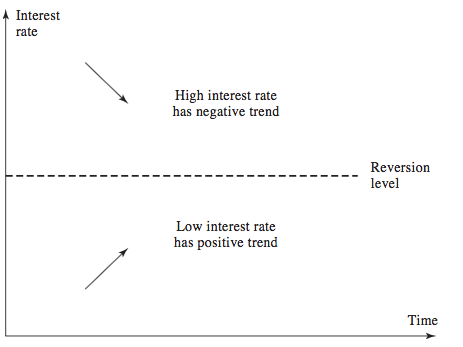
\includegraphics[width=0.8\textwidth]{img/meanreversion.png}
	\caption{Illustration of mean reversion}
	\label{fig:background:meanreversion}
	\source{Based on Options, Futures and Other Derivatives~\cite[pg. 684]{ofod}.}
\end{figure}

\subsection{Day-count Conventions}
% 28.8 https://en.wikipedia.org/wiki/Day_count_convention

Day-count conventions is a method for computing the amount of accrued interest, i.e. accumulated or received payments or benefits over time. It is usually used to asses the present value when the next coupon payment is less than a full coupon period away. Typically, bond markets and financial instruments have their own day-count conventions, which vary on the type of instrument, the interest rate type, and the issuance country. The standards were introduced to simplify accounting calculations and introduce constancy of time period, e.g. day, month, year. In the project, we chose to use Actual/365 Fixed method assuming the year to be 365 days and the actual differences to be calculated in days, i.e. the smallest interval is one day.

\subsection{Numerical Methods for Option Pricing}
%Numerical methods are mathematical tools typically designed to give an approximation on numerical problems. These include problems which either do not yet have an analytical solution (e.g. some differential equations cannot be solved exactly), or their analytical solutions take far too long to compute. A popular and useful numerical method for pricing options involves the construction of binomial or trinomial trees.~\cite[pg. 253]{ofod}

Numerical methods are mathematical tools designed to give approximate but accurate solutions to various numerical problems. Most often used methods are iterative methods that converge to a satisfactory result with a certain assumed level of approximation by iterating in a finite number of steps from the initial conditions. In this project, we deal with interpolation and solutions to continuous-time stochastic differential equations describing financial phenomena like interest rate. As we can only represent problems with finite amount of data, we need to discretize these problems by finding values in a finite number of points in a problem domain. We use numerical methods to solve problems that do not have an analytical solution, e.g. some differential equations cannot be solved exactly. While using numerical methods, it is important to address the numerical stability of the used algorithm to estimate and control round-off errors arising from the use of floating point arithmetic.

\paragraph{Binomial Tree}
 A most basic numerical method for pricing options involves the construction of trees or lattices.~\cite[pg. 253]{ofod} A binomial tree (see fig.~\ref{fig:background:binomtree}) is a numerical method, which allows to graphically represent the possible values that an option may take at different nodes or time periods. The value of the option depends on the underlying stock or bond, and computing values on the nodes is based on the probability that the price of the underlying asset will decrease or increase. The main advantage of binomial trees is that they are analytically tractable. This means that price valuation for a derivative can be performed on each node for every time step. This gives more flexibility and allows pricing of path-dependent derivatives, such as exotic options, having more complex cashflows. While the binomial model presented on fig. \ref{fig:background:binomtree} is unrealistically simple, the life of an option may in practice span for 30 or more time steps, making it possible to implicitly consider about $2^{30}$, or approx. 1 billion possible stock price paths.~\cite[pg. 268]{ofod}

\begin{figure}[H]
	\centering
	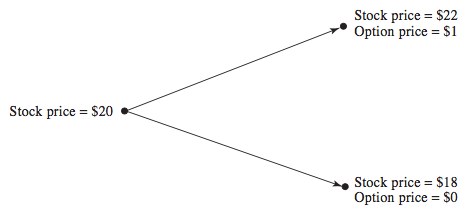
\includegraphics[width=0.8\textwidth]{img/binomtree.png}
	\caption{Illustration of a binomial tree}
	\label{fig:background:binomtree}
	\source{Based on Options, Futures and Other Derivatives~\cite[pg. 254]{ofod}.}
\end{figure}

% Chapter 20.4
\paragraph{Trinomial Tree}
The trinomial option pricing model (an example is shown on fig. \ref{fig:background:trinomtree}) is an alternative numerical method for constructing trees, with the difference that it consolidates another possible value per single time period. This makes the trinomial model even more relevant to real life situations, as it ensures the possibility that the value of the underlying asset may not change over a time period (taking the mid path on the tree). Calculations for a trinomial tree are analogous to those for a binomial tree.

\begin{figure}[H]
	\centering
	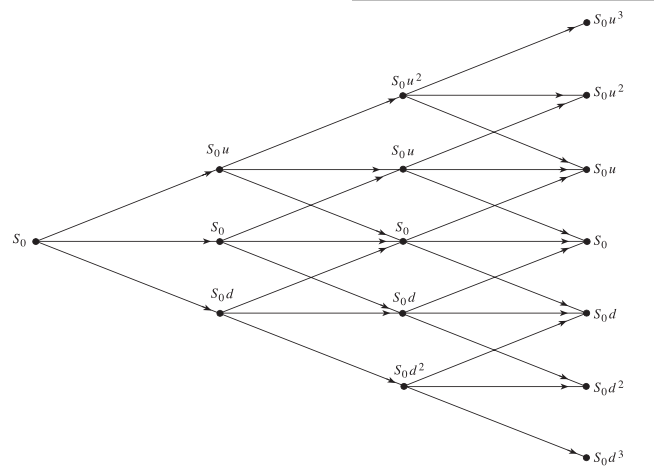
\includegraphics[width=0.8\textwidth]{img/trinomtree.png}
	\caption{Illustration of a trinomial tree}
	\label{fig:background:trinomtree}
	\source{Based on Options, Futures and Other Derivatives~\cite[pg. 444]{ofod}.}
\end{figure}

%Beside the Black-Scholes method and the binomial/trinomial tree approaches, there are yet other popular means for valuing derivatives. They have their advantages, but are either much more inefficient in terms of computation time, or perform similarly to trinomial trees. 

In this project, we use trinomial tree method as a numerical method for option pricing. However, there exist other methods that might be more suitable and performing better under certain specific conditions, that might be mathemtically and computationally more complex.

% 20.6 - Monte Carlo simulations
\paragraph{Monte Carlo simulations} samples different paths to obtain the expected payoff of the asset in a risk-neutral world and are then discounted at this risk-free rate. Monte Carlo Methods are particularly useful in the valuation of options with multiple sources of uncertainty (multiple dimensions) They are suitable for pricing instruments with complicated features, when the payoff depends on the path followed by the underlying variables, as this makes them difficult to value through a straightforward Black–Scholes analytical model or tree-based computation.  Unfortunately, the method is computationally intensive and might be too slow to be competitive over an analytical solution or other numerical techniques like trees. On the other hand, this constraint is less of concern in current computing environment with abundant and efficient compute capabilities. Another issue is that Monte Carlo procedures have to be adjusted to handle situations with early exercise opportunities, what increases their implementation complexity.~\cite[pg. 448]{ofod}  

% 20.8 - FDM
\paragraph{Finite difference methods (FDM)} value a derivative by solving the differential equation that the derivative satisfies. The differential equations are converted into sets of difference equations and are solved iteratively. This is similar to the trinomial trees method, since the computations also work back from the end of the derivative maturity to the beginning. In fact, tree based methods, if suitably parameterized, are a special case of the explicit finite difference method.~\cite[pg.455 - 466]{ofod} These type of methods can solve derivative pricing problems that have, in general, the same level of complexity as those problems solved by tree approaches, but, given their relative complexity, are usually employed only when other approaches are inappropriate. Furthermore, like tree-based methods, they are limited in terms of the number of underlying variables, i.e. multiple dimensions, they can handle.

%%%%% CUDA Background %%%%%
\newpage
\section{CUDA Background}
CUDA\footnote{Additional information about CUDA can be found on the Nvidia official documentation pages: \url{https://docs.nvidia.com/cuda/}}  is a parallel computing platform and a programming model based on C/C\texttt{++}, developed by Nvidia with the purpose to simplify and make GPGPU programming more accessible. It allows developers to incorporate various CUDA-specific keywords (such as e.g. \textit{\_\_device\_\_}, \textit{\_\_host\_\_}, \textit{cudaMemCpy}, \textit{blockIdx} and more.) into their programs, in order to express the parallelism and indicate to the compiler the code that should be run on the GPU.

\subsection{Process Flow}
CUDA allows the compiler to distinguish between serial and parallel code by using the \textit{\_\_host\_\_} and \textit{\_\_device\_\_} function modifiers respectively. While the first will be run as any other normal C/C\texttt{++} program on the CPU, the latter will be run on the GPU. Device functions can be called inside \textbf{kernel} functions that are defined with the \textit{\_\_global\_\_} keyword and when called, are executed $N$ times in parallel by $N$ different CUDA \textit{threads}. Since GPUs operate on their own memory, it is necessary that the input to the kernels is copied to the GPU memory beforehand. Furthermore, the results have to be copied back and both of these operations can be done with the use of the built-in \textit{cudaMemCpy()} function. Note that copying data back and forth from the GPU takes a rather high amount of time, hence GPU computing is not always suitable for all applications. It is often the case that the input is too small and it makes more sense to run an algorithm sequentially, as that will result in a shorter runtime. Return or temporary arrays must also be pre-allocated on the GPU beforehand, which is done by the \textit{cudaMalloc()} function.

Each parallel invocation of a kernel creates a CUDA \textbf{\textit{block}} of multiple \textbf{\textit{threads}} (currently up to 1024 threads). A \textit{block} executes only on one multiprocessor, which allows (i) synchronization (by means of barriers) across all \textit{threads} in the \textit{block} and (ii) the use of \textit{shared memory}, allowing \textit{threads} within a \textit{block} to communicate. On a larger scale, a set of \textit{blocks} is called a \textbf{\textit{grid}}. The number of blocks and threads can be specified by the programmer. A general overview of this structure is illustrated on fig.~\ref{fig:background:gridblockthread}.

\begin{figure}[H]
	\centering
	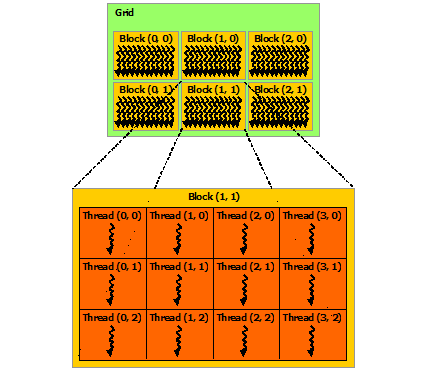
\includegraphics[width=.9\textwidth]{img/gridblockthread.png}
	\caption{Grid of Thread Blocks}
	\label{fig:background:gridblockthread}
\source{\url{https://docs.nvidia.com/cuda/cuda-c-programming-guide/}}
\end{figure}

CUDA automatically allocates \textit{thread blocks} and resources to the \textit{Streaming Multiprocessors} (\textit{SMs}). \textit{SMs} are the part of the GPU which runs the provided CUDA \textit{kernel} and they consist of several sub-components: \textit{Memory caches} (e.g. \textit{shared memory}, \textit{constant memory}, and more); thousands of \textit{registers}\footnote{\textit{Register memory} is memory allocated inside a single \textit{thread} and is only accessible by it through its lifespan. This is the fastest memory available in the CUDA memory model.}, which can be partitioned among the threads for execution; a \textit{warp scheduler}\footnote{When passed to the \textit{SM}, \textit{thread blocks} are split into \textit{warps} (currently with a maximum size of 32 \textit{threads}). All the \textit{threads} in a \textit{warp} execute concurrently on the resources of the \textit{SM}.} and \textit{execution cores} for both \textit{integer} and \textit{floating-point} operations. Fig.~\ref{fig:background:cudamemory} illustrates the CUDA memory model. 

\textit{Blocks} and \textit{threads} can be indexed inside the kernel in order to utilize the workload distribution among \textit{threads}. CUDA also allows the use of \textbf{\textit{shared memory}} between all threads within a block with the use of the \textit{\_\_shared\_\_} keyword, used when declaring arrays. In contrast to \textbf{\textit{global memory}}, which is accessible from all threads, \textit{shared memory} is much faster to operate with, due to its locality, as well as its different technology\footnote{\textit{Global memory} uses DRAM, while \textit{Shared memory} uses SRAM, which tends to be overclocked, hence faster.}.

The parallel access to data can often lead to \textit{data hazards}, such as \textit{RAW} (read after write), \textit{WAR} (write after read) or \textit{WAW} (write after write). While good software design can often help with \textit{data hazards} (i.e. as it will be seen in section~\ref{section:oneoption:seqtocuda}), it is often insufficient. In those situations, the \textit{\_\_syncthreads()} function can be called, which awaits all \textit{threads} within a \textit{block} and prevents incorrect memory reads/writes. Note that this slows down the overall runtime, thus it is up to the programmer to ensure it is only used when necessary.

\begin{figure}[H]
	\centering
	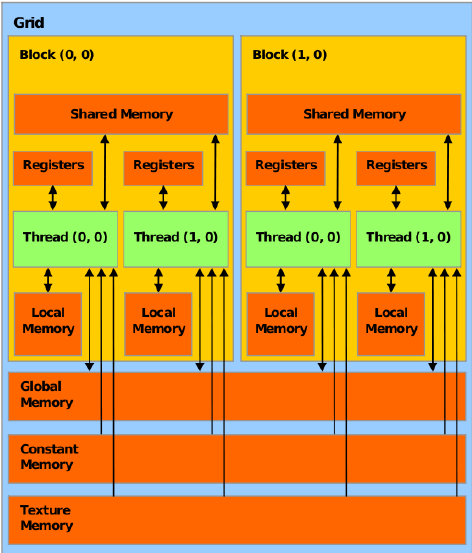
\includegraphics[width=.7\textwidth]{img/cudamemory.png}
	\caption{CUDA memory model}
	\label{fig:background:cudamemory}
	\source{Based on Nvidia CUDA Programming Guide 1.1, 2007}
\end{figure}

\subsection{Memory Coalescing}
One of the most significant hardware optimizations that CUDA provides is memory coalescing. It can be achieved when the threads in a warp access (when executing one read/write SIMD instruction) consecutive memory locations, making the access to be performed in one memory transaction. The consequences of not using memory coalescing can be as much as a warp different memory transaction to read/write this data. It is therefore important that the code is designed to take advantage of this optimization. As it can be seen on fig.~\ref{fig:background:memcoalescing}, an array can be restructured (transposed) allowing to take advantage of the order of elements. In the course of this project we have applied both coalesced and non-coalesced accesses and it has been interesting to observe the performance benefits it can lead to, as it will be shown in chapter \ref{chapter:experimentalresults}. 

\begin{figure}[H]
	\centering
	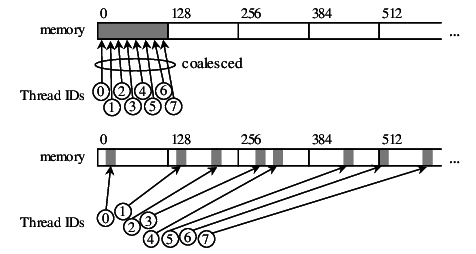
\includegraphics[width=.9\textwidth]{img/coalescing.png}
	\caption{Memory coalescing}
	\label{fig:background:memcoalescing}
\source{Based on Real-Time FFT Computation Using GPGPU for OFDM-Based Systems~\cite{rtfftcugpgpufobs}}
\end{figure}

\newpage
\section{Semantics and types of parallel operations}
To understand the flattening transformations applied and derive implementations exploiting different levels of flattening, it is necessary to first understand the higher-order functions we have used. Note that the functions described in this section can be redundant in imperative languages, such as CUDA. Despite that, parts of the work of this thesis is done in Futhark, hence these functions will be met throughout this report. For simplicity, these functions have been extracted from the Futhark language. Therefore this section will also serve as a ''Futhark background''. Note that for all functions below, $[n]\alpha$ denotes an array of $n$ elements of type $\alpha$ and $e$ denotes the neutral element.

\subsection{Zip and unzip}
\textit{Zip} and \textit{unzip} are used when working with tuples of data, as the first creates a tuple of values, while the latter can be used to extract the values of it. These functions are redundant in CUDA, however we have used them in the Futhark implementations. The signature of \textit{zip} is:
\begin{align}
  \nonumber&\mathit{zip}\;:\;[n]\alpha\rightarrow[n]\beta\rightarrow[n](\alpha, \beta)\\
  \nonumber&\mathit{zip}\;[x_1, x_2, ... x_n]\;[y_1, y_2, ... y_n]=[(x_1, y_1),(x_2, y_2)...,(x_n, y_n)]
\end{align}
Conversely, the signature of \textit{unzip} is:
\begin{align}
  \nonumber&\mathit{unzip}\;:\;[n](\alpha, \beta)\rightarrow([n]\alpha,[n]\beta)\\
  \nonumber&\mathit{unzip}\;[(x_1, y_1),(x_2, y_2)...,(x_n, y_n)]=([x_1, x_2, ... x_n],[y_1, y_2, ... y_n])
\end{align}

\subsection{Map}
A \textit{map} applies a given function to each element of a list. It therefore takes a function and an array as input. It has the following signature:

\begin{align}
  \nonumber&\mathit{map}\;:\;(\alpha\rightarrow\beta)\rightarrow [n]\alpha\rightarrow[n]\beta\\
  \nonumber&\mathit{map}\;f\;[x_1,x_2,...,x_n]=[f(x_1),f(x_2),...,f(x_n)]
\end{align}
We have additionally used \textit{map2}, \textit{map3} and similar \textit{map} variations in Futhark, which have different signatures than the ones above, where the map is applied to multiple arrays (\textit{map2} for 2, \textit{map3} for 3, etc.) of the same size. In these cases, the function $f$ takes multiple parameters, one from each array. For simplicity, we have used only \textit{map} in our pseudo-code, even though the maps may take multiple arrays as input. In these cases, the number of arguments in the lambda function indicate the number of input arrays if unclear.   

\subsection{Reduce}
A \textit{reduce} uses a given binary-associative operator, a neutral element, and an array, and it recursively accumulates the array elements with the combining operator, starting with the neutral element, building up the return value. \textit{Reduce} is quite similar to a \textit{scan} (discussed in the next subsection), with the only difference that it does not keep intermediate values. The function has the following signature:

\begin{align}
  \nonumber&\mathit{reduce}\;:\;(\alpha\rightarrow\alpha\rightarrow\alpha)\rightarrow\alpha\rightarrow[n]\alpha\rightarrow\alpha\\
  \nonumber&\mathit{reduce}\;\odot\;e\;[x_1,x_2,...,x_n]=e\odot x_1\odot x_2\odot ...\odot x_n
\end{align}
We have created an alias for \textit{reduce}, named \textit{reducePlus}, which corresponds to $\mathit{reduce}\;(+)\;0$ where the combining operator is $+$ and $0$ is the neutral element.

\subsection{Scan}
An \textit{inclusive scan} (or just \textit{scan}) uses a given binary-associative operator, a neutral element, and an array and recursively accumulates the array elements with the combining operator, starting with the neutral element, building up the return values. Note that (i) \textit{scan} returns an array containing all intermediate values, differently from \textit{reduce} and (ii) the neutral element is not returned together with the intermediate values. Another variation of \textit{scan} is \textit{exclusive scan}/\textit{scanExc}, which shifts the return array of a typical \textit{scan} to the left with one element, including the neutral element in the beginning and excluding the last element (hence the name exclusive). \textit{Scan} (inclusive) has the following signature:

\begin{align}
  \nonumber&\mathit{scan}\;:\;(\alpha\rightarrow\alpha\rightarrow\alpha)\rightarrow\alpha\rightarrow[n]\alpha\rightarrow[n]\alpha\\
  \nonumber&\mathit{scan}\;\odot\;e\;[x_1,x_2,...,x_n]=[e\odot x_1,...,e\odot x_1\odot...\odot x_n]
\end{align}
while an exclusive scan has the signature:
\begin{align}
  \nonumber&\mathit{scanExc}\;:\;(\alpha\rightarrow\alpha\rightarrow\alpha)\rightarrow\alpha\rightarrow[n]\alpha\rightarrow[n]\alpha\\
  \nonumber&\mathit{scanExc}\;\odot\;e\;[x_1,x_2,...,x_n]=[e,e\odot x_1,...,e\odot x_1\odot...\odot x_{n-1}]
\end{align}
\textit{Scan} has been one of the most used functions in this project. To reduce redundancy in the pseudo-code of the following chapters, we have created an alias for it - \textit{scanPlus}, which corresponds to $\mathit{scan}\;(+)\;0$ where the combining operator is $+$ and $0$ is the neutral element.

\subsection{Segmented scan}
A two-dimensional irregular array --- meaning the rows (segments) do not have the same lengths --- can be represented by a flat array of values of primitive types together with a ``flag'' array, which denotes where each row (segment) starts---in essence a {\tt true} or {\tt 1} flag value denotes the start of a new segment and a {\tt false} or {\tt 0} value denotes that the current element is within a segment but not the first element of the segment. A \textit{segmented scan}/\textit{sgmScan} operator semantically performs in parallel an inclusive scan on each of the segments of the array.  (Note that exclusive scan can also be segmented, but it will not be introduced, as it was not used in this thesis).
\textit{Segmented scan} has a type similar to \textit{scan}, except that it also receives the flag array as parameter; moreover it is also straightforwardly implemented by means of \textit{scan}. Its type and implementation are presented below:
\begin{align}
  \nonumber&\mathit{sgmScan}\;:\;(\alpha\rightarrow\alpha\rightarrow\alpha)\rightarrow\alpha\rightarrow[n]\mbox{\tt bool}\rightarrow[n]\alpha\rightarrow[n]\alpha\\
  \nonumber&\mathit{sgmScan}\;\odot\;e\;\mathit{flags}\;\mathit{vals}=\\
  \nonumber&\mbox{\tt~~}let~(\_,\mathit{vals'})~=~\mathit{scan}~(\ (f_1,v_1)~(f_2,v_2)~\rightarrow\\
  \nonumber&\mbox{\tt~~~~~~~~~~~~~~~~~~~~~~~} \mbox{\tt if}~f_2~\mbox{\tt then}~(\mbox{\tt true},v_2)~\mbox{\tt else}~(f_1~\mbox{\tt ||}~f_2,~v_1~\odot~v_2)\\
  \nonumber&\mbox{\tt~~~~~~~~~~~~~~~~~~~~} )~(\mbox{\tt false},e)~(\mbox{\tt zip}~flags~vals)\\
  \nonumber&\mbox{\tt~~in}~\mathit{vals'}
\end{align}
%%  \nonumber&sgmScan\;\odot\;e\;[b_1,b_2,...,b_n]\;[x_1_1,x_1_2,x_n_1,...,x_n_m]\\
%  \nonumber&=[e\odot x_1_1, e\odot x_1_1\odot x_1_2,e\odot x_n_1,e\odot x_n_1\odot...\odot x_n_m]
Similar to \textit{scanPlus} and \textit{reducePlus}, we have also created an alias for \textit{sgmScan} - \textit{sgmScanPlus}, which corresponds to $\mathit{sgmScan}\;(+)\;0$ where the combining operator is $+$ and $0$ is the neutral element.

\subsection{Replicate}
\textit{Replicate} takes an integer \textit{n} and a value \textit{m} and creates an array of length \textit{n} whose elements have value \textit{m}. The function signature is:

\begin{align}
  \nonumber&\mathit{replicate}\;:\;(n:int)\rightarrow\beta\rightarrow [n] \beta\\
  \nonumber&\mathit{replicate}\;n\;m=[m,...,m]
\end{align}

\subsection{Scatter}
\textit{Scatter} is used for bulk in-place updates with multiple values and takes an array to write to, an array of indexes showing which elements of the first arrays should be updated, and an array of values, i.e. the updates. Note that CUDA supports in-place updates, hence this operation is not needed. The signature is shown below:
\begin{align}
  \nonumber&\mathit{scatter}\;:\;[n]\alpha\rightarrow[m]\beta\rightarrow [m]\alpha\rightarrow [n]\alpha
%  \nonumber&scatter\;[x_1,x_2,...x_n]\;[i_1,i_2...,i_m]\;[v_1,v_2...,v_m]\\
%  \nonumber&=map\;(i\rightarrow\;if\;(i > -1)\;then (x[i]=v_i))\;[i_1,i_1,...,i_m]
\end{align}

\subsection{Iota}
The \textit{iota} function is Futhark-specific and is used to create an array of index values, used to map indexes over elements. It takes an integer as input. The signature is shown below:
\begin{align}
  \nonumber&\mathit{iota}\;:\;(n:int)\rightarrow[n]\mathit{int}\\
  \nonumber&\mathit{iota}\;n=[0,1...,n-1]
\end{align}
\subsection{Last}
\textit{Last} takes an array as input and returns the last element of it. The signature is:
\begin{align}
  \nonumber&\mathit{last}\;:\;[n]\alpha\rightarrow\alpha\\
  \nonumber&\mathit{last}\;[x_1, x_2, ... x_n]=x_n
\end{align}
\subsection{Length}
\textit{Length} takes an array as input and returns its length/size. The signature is:
\begin{align}
  \nonumber&\mathit{length}\;:\;[n]\alpha\rightarrow int\\
  \nonumber&\mathit{length}\;[x_1, x_2, ... x_n]=n
\end{align}

\newpage
%%%% FLATTENING BACKGROUND %%%%
\section{Flattening Background}
\label{chapter:section:flattening}
As briefly mentioned in the Introduction, complex applications are often composed of multiple nested levels of operations. This means that operations are often performed on nested arrays such as $a=[[1,2],[3,4,5],[6,7,8,9]]$. Suppose that we want to apply the function $f(x)=x+1$ to each element in the array (note that iteration over arrays is done via a map). This cannot be done directly, as $x$ is of type ''array of integers''. Instead, we can iterate over all nested arrays (with the use of another \textit{map}) and apply the function to each sub-array as follows: $\mathit{map}\;(\backslash x\rightarrow \mathit{map}\;f(x))\;a$. In order to effectively utilize massively parallel hardware, it is necessary that nested higher-order functions (such as \textit{map}, \textit{scan}, \textit{reduce}, etc.) are flattened, so that they can operate on flat arrays. Their
transformation can be done through certain flattening techniques such as the ones described in this section. Flattening an array itself is straightforward, as the example above becomes $\mathit{flat\_a}=[1,2,3,4,5,6,7,8,9]$. Albeit, the flattened representation of an array does not contain any indication of how many nested arrays existed before, nor on their separation. Hence it is often necessary to introduce additional arrays such as \textit{shape} and \textit{flags}. In our example, $\mathit{shape\_a}=[2,3,4]$, contains the length of each sub-array of $a$. Denoting the length of \textit{shape\_a} by $m$ and the length of \textit{flat\_a} by $n$, we can create the \textit{flag} array by:

\begin{itemize}
    \item using an exclusive scan to compute the indices where a {\tt true} or {\tt 1} value should be placed in the flag array, i.e., $\mathit{inds}~=~\mathit{scanExc}\;(+)\;0\;\mathit{shape\_a}~=~[0,2,5]$,
    \item updating an array of {\tt false} values with {\tt true} at the computed indices, i.e., $\mathit{flags\_a}~=~\mathit{scatter}\;(\mathit{replicate}~n~\mbox{\tt false})\;\mathit{inds}\;(\mathit{replicate}\;m\;\mbox{\tt{}true})$ which results in $[1,0,1,0,0,1,0,0,0]$.
\end{itemize}

The flag array can be later used to flatten nested operations, for example in the case of segmented scan. Note that only the flattening transformations that have been used in this project are described, even though many more transformations can be devised. Note also that these transformations are only guidelines and they can be simplified in practice, as some of the steps may be redundant in various combinations of operations. 

\subsection{Nested Map in a Map}
\label{chapter:section:flattening:map}
 A nested map inside a map is one of the simplest flattening transformations that can be performed. The procedure is as simple as applying the nested map on the flattened array, meaning that:
\begin{equation}
\centering
\nonumber
\mathit{map}\;(x\rightarrow \mathit{map}\;f(x))\;a\;\equiv\;\mathit{map}\;(x\rightarrow f(x))\;\mathit{flat\_a}
\end{equation}
Applying the map to the flat array shown as an example in the beginning of this section, we get $\mathit{map}\;(x\rightarrow x + 1)\;[1,2,3,4,5,6,7,8,9]=[2,3,4,5,6,7,8,9,10]$

\subsection{Nested Scan in a Map}
\label{chapter:section:flattening:scan}
Flattening \textit{scan} is also done in a single step, as it is replaced with a \textit{segmented scan}, taking an additional \textit{flags} array. In general, the flattening transformation of a nested \textit{scan} can be described as (where $e$ is the neutral element):
\begin{equation}
\centering
\nonumber
\mathit{map}\;(x\rightarrow \mathit{scan}\;\odot\;e\;x)\;a\;
\equiv\;
\mathit{sgmScan}\;\odot\;e\;\mathit{flags\_a}\;\mathit{flat\_a}
\end{equation}
Using the array $a$ mentioned previously as an example, $(+)$ as a cumulative operator and $0$ as a neutral element, we can apply\\ $\mathit{sgmScan}\;(+)\;0\;[1,0,1,0,0,1,0,0,0]\;[1,2,3,4,5,6,7,8,9]\;=[1,3,3,7,12,6,13,21,30]$ 

\subsection{Nested Replicate in a Map}
\label{chapter:section:flattening:replicate}
As previously mentioned, replicate takes as inputs an integer and a value of some arbitrary type $\alpha$. For simplicity (only in this section), we will name them \textit{n} and \textit{x}, where \textit{n} is the number of times \textit{x} should be replicated. The flattening of a \textit{replicate} nested inside a \textit{map} becomes a combination of scans and scatters. In the following we assume the flat array $a$ is of type $[q](\mathit{int},\alpha)$:
\begin{equation}
\centering
\nonumber
\mathit{map}\;(\backslash(n,x)\rightarrow \mathit{replicate}\;n\;x)\;a\;
\equiv\; \mathit{sgmScanInc}\;(+)\;0\;\mathit{flags}\;\mathit{vals}
\end{equation}
where:\\
$(\mathit{shape},\mathit{xs})~=~\mathit{unzip}~a$\\
$\mathit{inds}~=~\mathit{scanExc}\;(+)\;0\;\mathit{shape}$\\
$\mathit{flatlen}~=~(\mathit{last}\;\mathit{inds})\;+\;(\mathit{last}\;\mathit{shape})$\\
$\mathit{flags}~=~\mathit{scatter}\;(\mathit{replicate}\;\mathit{flatlen}\;\mbox{\tt false})\;\mathit{inds}\;(\mathit{replicate}~n~\mbox{\tt true})$\\
$\mathit{vals}~=~\mathit{scatter}\;(\mathit{replicate}\;\mathit{flatlen}\;\mbox{\tt false}))\;\mathit{inds}\;\mathit{xs}$\\

The above re-write rule says that a replicate operation nested in a map will generate a flat array (by means of the \textit{sgmScan} operation), whose structure is described by the \textit{shape} (and \textit{flags}) arrays. Since the re-write rule is very dry, we work an example by hand to provide more insight.

Suppose that we have a $\mathit{map}\;((n,x)\rightarrow \mathit{replicate}\;n\;x)\;[(1,7), (3,8), (2,9)]$, that is, to replicate $7$ one time, $8$ three times, and $9$ two times through the iterations of the map. We start by deriving \\
$(\mathit{shape},\;\mathit{xs})=\mathit{unzip}([(1,7),(3,8),(2,9)])=([1,3,2],[7,8,9])$\\
$\mathit{inds}=\mathit{scanExc}\;(+)\;0\;[1,3,2]=[0,1,4]$\\
$\mathit{flatlen}=(\mathit{last}\;[0,1,4])+(\mathit{last}\;[1,3,2])=4+2=6$\\
$\mathit{flags}=\mathit{scatter}\;[0,0,0,0,0,0]\;[0,1,4]\;[1,1,1]=[1,1,0,0,1,0]$\\
$\mathit{vals}=\mathit{scatter}\;[0,0,0,0,0,0]\;[0,1,4]\;[7,8,9]=[7,8,0,0,9,0]$\\
and finally\\
$\mathit{sgmReplicate}=\mathit{sgmScan}\;(+)\;0\;[1,1,0,0,1,0]\;[7,8,0,0,9,0]=[7,8,8,8,9,9]$

\subsection{Nested Reduce inside a Map}
\label{chapter:section:flattening:reduce}

We cover now the case in which a reduce is nested inside a map:\\
$\mbox{~~~~~~~~~~~}\mathit{map}~(\backslash x~\rightarrow~\mathit{reduce}~\odot~e~x)~a$\\
where $a$ is a two-dimensional irregular array, represented by (1) array \textit{flat\_a}, which holds the flattened values, and by (2) arrays \textit{shape\_a} and \textit{flat\_a} which encode the row structure of $a$, as explained before.

The result of flattening is a flat array containing as many elements as rows in $a$ (i.e., length of \textit{shape\_a}), in which each element of the result is obtained by reducing the corresponding segment with the given operator and neutral element, a.k.a. segmented reduce. The re-write rule is given below (and it assumes no empty rows):
\begin{equation}
\centering
\nonumber
\mathit{map}\;(\backslash x\rightarrow \mathit{reduce}\;\odot\;e\;x)\;a\;
\equiv\;
\mathit{map}\;(\backslash i\;\rightarrow\;\mathit{vals}[i-1])\;\mathit{shape\_scanned}
\end{equation}
where\\
$\mathit{shape\_scanned}\;=\;\mathit{scan}\;\odot\;e\;\mathit{shape\_a}$\\
$\mathit{vals}\;=\;\mathit{sgmScan}\;(\odot)\;e\;\mathit{flags\_a}\;\mathit{flat\_a}$\\

Suppose that we simplify the example in the beginning of this section, such that $\odot=+$, $e=0$, $a=[[1,2],[3,4,5]]$; $\mathit{flat\_a}=[1,2,3,4,5]$; $\mathit{shape\_a}=[2,3]$, and $\mathit{flags\_a}=[1,0,1,0,0]$. Then the segmented reduce is obtained as follows:\\\\
$\mathit{shape\_scanned}\;=\;\mathit{scan}\;(+)\;0\;\mathit{shape\_a}\;=\;[2,5]$\\
$\mathit{vals}\;=\;\mathit{sgmScan}\;(+)\;0\;[1,0,1,0,0]\;[1,2,3,4,5]=[1,3,3,7,12]$\\
and finally\\
$\mathit{sgmReduce}\;=\;\mathit{map}\;(\backslash i\;\rightarrow\;\mathit{vals}[i-1])\;\mathit{shape\_scanned}\;=\;[3,12]$

\section*{Summary}
% This chapter has provided a brief introduction to to the necessary knowledge needed to understand the following chapters. This has covered financial topics such as options, volatility, trinomial trees, and more, all needed in the implementations. Following was an introduction to the basics needed for understanding terminology and techniques in CUDA, which have been used throughout this thesis. Next, this chapter has covered the parallel operations used in the thesis, immediately followed by the flattening background needed for applying transformations in order to exploit thread divergence and experiment with different levels of nested parallelism. The following chapter will study the Hull-White Single-Factor Model, in order to explore its mechanisms and prepare an implementation strategy.

This chapter has provided a brief introduction to the necessary concepts mentioned in the consequent chapters. It has covered financial topics such as options, volatility, numerical methods, and more, all needed in the implementations. Following was an introduction to the basics needed for understanding terminology and techniques in CUDA, which have been used throughout this thesis. Next, this chapter has covered the parallel operations used in the thesis, immediately followed by the flattening background needed for applying transformations in order to exploit thread divergence and experiment with different levels of nested parallelism. 